\vspace{0.15cm}
\begin{flushleft}
	{\color{blue!50!green}\fbox{\fontfamily{qag}\bfseries\selectfont PHẦN I. Câu trắc nghiệm nhiều phương án lựa chọn (3,0 điểm)}}
	\textit{\small (Thí sinh trả lời từ câu 1 đến câu 12. Mỗi câu hỏi thí sinh chỉ chọn một phương án.)}
\end{flushleft}
\setcounter{ex}{0}
\setcounter{bt}{0}

% Câu 1
\begin{ex}
	\macau{ID: VL12-QH2526-C01}Đơn vị của nội năng là
	\choice
	{Vôn ($\text{V}$)}
	{Oát ($\text{W}$)}
	{\True Jun ($\text{J}$)}
	{Niu-tơn ($\text{N}$)}
	\loigiai{
		Nội năng là một dạng năng lượng nên có đơn vị đo trong hệ SI là Jun ($\text{J}$)}
\end{ex}

% Câu 2
\begin{ex}
	\macau{ID: VL12-QH2526-C02}Chất khí dễ nén hơn chất lỏng và chất rắn vì
	\choice
	{phân tử khí chuyển động nhanh hơn phân tử lỏng và rắn}
	{phân tử khí có kích thước nhỏ hơn phân tử lỏng và rắn}
	{lực liên kết giữa các phân tử khí mạnh hơn chất lỏng và chất rắn}
	{\True khoảng cách giữa các phân tử khí lớn hơn nhiều so với chất lỏng và chất rắn}
	\loigiai{
		Ở thể khí, khoảng cách giữa các phân tử rất lớn so với kích thước của chúng và so với thể lỏng, thể rắn, do đó chất khí rất dễ bị nén}
\end{ex}

% Câu 3
\begin{ex}
	\macau{ID: VL12-QH2526-C03}Khi hai vật có nhiệt độ chênh lệch tiếp xúc nhau thì nhiệt năng
	\choice
	{\True truyền từ vật có nhiệt độ cao sang vật có nhiệt độ thấp}
	{truyền từ vật có nhiệt độ thấp sang vật có nhiệt độ cao}
	{hai vật ở trạng thái cân bằng nhiệt}
	{không có sự truyền nhiệt năng giữa chúng}
	\loigiai{
		Nhiệt năng tự truyền từ vật có nhiệt độ cao hơn sang vật có nhiệt độ thấp hơn cho đến khi đạt trạng thái cân bằng nhiệt}
\end{ex}

% Câu 4
\begin{ex}
	\macau{ID: VL12-QH2526-C04}Phát biểu nào sau đây \textbf{không đúng} khi nói về nhiệt nóng chảy riêng của chất?
	\choice
	{Được đo bằng đơn vị $\text{J/kg}$}
	{Nhiệt lượng trong quá trình truyền nhiệt để làm vật nóng chảy hoàn toàn ở nhiệt độ nóng chảy là: $Q = m\lambda$}
	{\True Các chất khác nhau có khối lượng bằng nhau thì có nhiệt nóng chảy riêng như nhau}
	{Nhiệt nóng chảy riêng của một chất là nhiệt lượng cần để làm cho $1\text{ kg}$ chất đó nóng chảy hoàn toàn ở nhiệt độ nóng chảy}
	\loigiai{
		Nhiệt nóng chảy riêng $\lambda$ là đặc trưng cho bản chất của từng chất nóng chảy, các chất khác nhau thì có nhiệt nóng chảy riêng khác nhau. Do đó phát biểu C là không đúng}
\end{ex}

% Câu 5
\begin{ex}
	\macau{ID: VL12-QH2526-C05}Một lượng khí bị nén đã nhận được công là $120\text{ kJ}$. Khí nóng lên và đã tỏa nhiệt lượng $70\text{ kJ}$ ra môi trường. Độ biến thiên nội năng của lượng khí này là
	\choice
	{$190\text{ kJ}$}
	{$-50\text{ kJ}$}
	{\True $50\text{ kJ}$}
	{$-190\text{ kJ}$}
	\loigiai{
		Khí nhận công nên $A = 120\text{ kJ}$.\\
		Khí tỏa nhiệt lượng nên $Q = -70\text{ kJ}$.\\
		Theo định luật I nhiệt động lực học:
		\[
		\Delta U = A + Q = 120 + (-70) = 50\text{ kJ}.
		\]
	}
\end{ex}

% Câu 6
\begin{ex}
	\macau{ID: VL12-QH2526-C06}Một cục nước đá rất lớn ở $t_1 = 0^\circ\text{C}$ có một cái hốc với thể tích $V_0 = 160\text{ cm}^3$. Người ta rót vào hốc đó $m_n = 80\text{ g}$ nước ở nhiệt độ $t_2^\circ\text{C}$. Cho biết khối lượng riêng của nước $D_n = 1000\text{ kg/m}^3 = 1\text{ g/cm}^3$ và nước đá là $D_{da} = 900\text{ kg/m}^3 = 0{,}9\text{ g/cm}^3$, nhiệt dung riêng của nước $c = 4200\text{ J/(kg}\cdot\text{K)}$, nhiệt nóng chảy riêng của nước đá $\lambda = 3{,}36 \times 10^5\text{ J/kg}$. Khi hốc nước nguội hẳn thì thể tích hốc rỗng còn lại là $88\text{ cm}^3$. Giá trị nhiệt độ $t_2$ là
	\choice
	{$7{,}2^\circ\text{C}$}
	{$67^\circ\text{C}$}
	{\True $72^\circ\text{C}$}
	{$9{,}3^\circ\text{C}$}
	\loigiai{
		Vì cục nước đá rất lớn nên nhiệt độ cuối cùng của hệ là $0^\circ\text{C}$.\\
		Nhiệt lượng do $80\text{ g} = 0{,}08\text{ kg}$ nước tỏa ra để hạ nhiệt độ từ $t_2$ xuống $0^\circ\text{C}$:
		\[
		Q_{tỏa} = m_n c (t_2 - 0) = 0{,}08 \times 4200 \times t_2 = 336 t_2\text{ (J)}.
		\]
		Nhiệt lượng này làm tan chảy một lượng nước đá có khối lượng $\Delta m$ ở $0^\circ\text{C}$:
		\[
		Q_{thu} = \Delta m \cdot \lambda = \Delta m \times 3{,}36 \times 10^5\text{ (J)}.
		\]
		Khi một lượng nước đá khối lượng $\Delta m$ tan chảy:
		\begin{itemize}
			\item Thể tích của hốc tăng thêm một lượng bằng thể tích khối đá bị tan: $\Delta V_{hốc} = \dfrac{\Delta m}{D_{da}}$.
			\item Lượng đá tan biến thành nước có thể tích: $V_{n, mới} = \dfrac{\Delta m}{D_n}$.
		\end{itemize}
		Tổng thể tích nước có trong hốc lúc cân bằng nhiệt (gồm nước ban đầu và nước đá tan):
		\[
		V_{n, tổng} = \dfrac{m_n + \Delta m}{D_n}.
		\]
		Thể tích hốc lúc sau: $V_{hốc, sau} = V_0 + \dfrac{\Delta m}{D_{da}}$.\\
		Thể tích phần hốc rỗng còn lại:
		\[
		V_{rỗng} = V_{hốc, sau} - V_{n, tổng} = V_0 + \dfrac{\Delta m}{D_{da}} - \dfrac{m_n + \Delta m}{D_n} = V_0 - \dfrac{m_n}{D_n} + \Delta m \left(\dfrac{1}{D_{da}} - \dfrac{1}{D_n}\right).
		\]
		Thay các số liệu vào ($V$ tính theo $\text{cm}^3$, khối lượng tính theo $\text{g}$):
		\[
		88 = 160 - \dfrac{80}{1} + \Delta m \left(\dfrac{1}{0{,}9} - 1\right) = 80 + \dfrac{\Delta m}{9} \Rightarrow \dfrac{\Delta m}{9} = 8 \Rightarrow \Delta m = 72\text{ g} = 0{,}072\text{ kg}.
		\]
		Theo phương trình cân bằng nhiệt:
		\[
		336 t_2 = 0{,}072 \times 3{,}36 \times 10^5 = 24\,192 \Rightarrow t_2 = \dfrac{24\,192}{336} = 72^\circ\text{C}.
		\]
	}
\end{ex}

% Câu 7
\begin{ex}
	\immini{
	\macau{ID: VL12-QH2526-C07}Để xác định nhiệt dung riêng của nước bằng thí nghiệm sách giáo khoa trình bày thì \textbf{không cần đo} đại lượng nào sau đây?
	\choice
	{\True Cường độ dòng điện}
	{Công suất dòng điện}
	{Thời gian đun nước}
	{Nhiệt độ nước sau khi đun}
	}{
	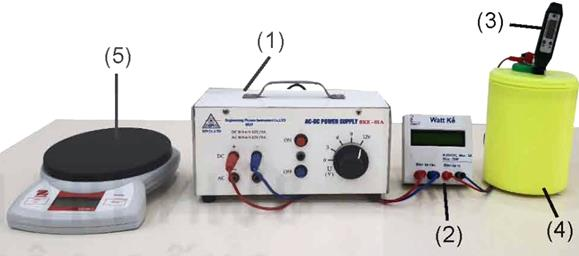
\includegraphics[width=4.5cm]{figures/fig_page1.png}
	}
	\loigiai{
		Trong sơ đồ thí nghiệm xác định nhiệt dung riêng của nước, người ta sử dụng oát kế (Watt kế) để đo trực tiếp công suất điện $P$ cung cấp cho nhiệt lượng kế, đồng hồ đo thời gian $t$, nhiệt kế đo nhiệt độ và cân điện tử đo khối lượng nước.\\
		Do đã có công suất $P$, ta tính được nhiệt lượng $Q = P \cdot t$ mà không cần phải đo trực tiếp cường độ dòng điện $I$}
\end{ex}

% Câu 8
\begin{ex}
	\macau{ID: VL12-QH2526-C08}Sự chuyển thể từ rắn sang lỏng được gọi là
	\choice
	{sự thăng hoa}
	{sự ngưng tụ}
	{\True sự nóng chảy}
	{sự bay hơi}
	\loigiai{
		Quá trình chuyển từ thể rắn sang thể lỏng được gọi là sự nóng chảy}
\end{ex}

% Câu 9
\begin{ex}
	\macau{ID: VL12-QH2526-C09}Biết nhiệt dung riêng của nước là $4200\text{ J/(kg}\cdot\text{K)}$, nhiệt hóa hơi riêng của nước ở $100^\circ\text{C}$ là $2{,}26 \times 10^6\text{ J/kg}$. Nhiệt lượng cần thiết để làm cho $1\text{ kg}$ nước ở $30^\circ\text{C}$ chuyển hoàn toàn thành hơi nước ở $100^\circ\text{C}$ là
	\choice
	{$25540\text{ kJ}$}
	{\True $2554\text{ kJ}$}
	{$255400\text{ J}$}
	{$25{,}54\text{ J}$}
	\loigiai{
		Nhiệt lượng cần để nâng nhiệt độ của $1\text{ kg}$ nước từ $30^\circ\text{C}$ lên $100^\circ\text{C}$:
		\[
		Q_1 = m c (100 - 30) = 1 \times 4200 \times 70 = 294\,000\text{ J}.
		\]
		Nhiệt lượng cần để làm $1\text{ kg}$ nước hóa hơi hoàn toàn ở $100^\circ\text{C}$:
		\[
		Q_2 = m L = 1 \times 2{,}26 \times 10^6 = 2\,260\,000\text{ J}.
		\]
		Tổng nhiệt lượng cần cung cấp:
		\[
		Q = Q_1 + Q_2 = 294\,000 + 2\,260\,000 = 2\,554\,000\text{ J} = 2554\text{ kJ}.
		\]
	}
\end{ex}

% Câu 10
\begin{ex}
	\immini{
	\macau{ID: VL12-QH2526-C10}Có 4 bình A, B, C, D đều đựng nước ở cùng một nhiệt độ với thể tích tương ứng là: $1\text{ lít}$, $2\text{ lít}$, $3\text{ lít}$, $4\text{ lít}$. Sau khi dùng các đèn cồn giống hệt nhau để đun các bình này trong cùng một khoảng thời gian (đến khi nước chưa sôi) thì bình nào có nhiệt độ cao nhất?
	\choice
	{Bình B}
	{Bình D}
	{\True Bình A}
	{Chưa đủ giả thiết để xác định}
	}{
	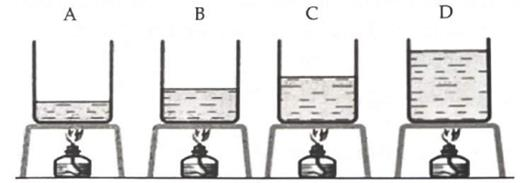
\includegraphics[width=4.5cm]{figures/fig_page2.png}
	}
	\loigiai{
		Trong cùng một khoảng thời gian, các đèn cồn giống hệt nhau cung cấp cùng một lượng nhiệt $Q$.\\
		Độ tăng nhiệt độ của nước trong mỗi bình: $\Delta t = \dfrac{Q}{m c}$.\\
		Vì nhiệt dung riêng $c$ và lượng nhiệt $Q$ như nhau nên bình nào có khối lượng nước nhỏ nhất sẽ có độ tăng nhiệt độ lớn nhất, do đó đạt nhiệt độ cao nhất.\\
		Bình A chứa ít nước nhất ($1\text{ lít}$) nên sẽ có nhiệt độ cao nhất}
\end{ex}

% Câu 11
\begin{ex}
	\macau{ID: VL12-QH2526-C11}Nhiệt hóa hơi riêng của nước là $2{,}26 \times 10^6\text{ J/kg}$ có nghĩa là
	\choice
	{$1\text{ kg}$ nước cần thu nhiệt lượng $2{,}26 \times 10^6\text{ J}$ để hóa lỏng}
	{$1\text{ kg}$ nước sẽ tỏa ra nhiệt lượng $2{,}26 \times 10^6\text{ J}$ khi hóa hơi hoàn toàn}
	{\True $1\text{ kg}$ nước cần thu nhiệt lượng $2{,}26 \times 10^6\text{ J}$ khi hóa hơi hoàn toàn ở nhiệt độ xác định}
	{$1\text{ kg}$ nước tỏa ra nhiệt lượng $2{,}26 \times 10^6\text{ J}$ khi hóa hơi hoàn toàn}
	\loigiai{
		Nhiệt hóa hơi riêng của một chất là nhiệt lượng cần cung cấp cho $1\text{ kg}$ chất lỏng đó để nó hóa hơi hoàn toàn ở nhiệt độ sôi xác định. Do đó $1\text{ kg}$ nước cần thu nhiệt lượng $2{,}26 \times 10^6\text{ J}$ để hóa hơi hoàn toàn ở nhiệt độ sôi}
\end{ex}

% Câu 12
\begin{ex}
	\macau{ID: VL12-QH2526-C12}Nhiệt hóa hơi riêng được kí hiệu là
	\choice
	{\True $L$}
	{$Q$}
	{$\lambda$}
	{$c$}
	\loigiai{
		Nhiệt hóa hơi riêng được kí hiệu là $L$ (trong một số tài liệu có thể dùng $L$ hoặc $r$). Nhiệt nóng chảy riêng kí hiệu là $\lambda$, nhiệt dung riêng kí hiệu là $c$, nhiệt lượng kí hiệu là $Q$}
\end{ex}

\vspace{0.15cm}
\begin{flushleft}
	{\color{blue!50!green}\fbox{\fontfamily{qag}\bfseries\selectfont PHẦN II. Câu trắc nghiệm Đúng/Sai (2,0 điểm)}}
	\textit{\small (Thí sinh trả lời từ câu 1 đến câu 2. Trong mỗi ý a), b), c), d) ở mỗi câu, thí sinh chọn đúng hoặc sai.)}
\end{flushleft}
\setcounter{ex}{0}

% Câu 13
\begin{ex}
	\macau{ID: VL12-QH2526-C13}Một học sinh làm thí nghiệm đun nóng để làm $1\text{ kg}$ nước đá (thể rắn) ở $0^\circ\text{C}$ chuyển hoàn toàn thành hơi nước ở $100^\circ\text{C}$. Cho nhiệt nóng chảy của nước ở $0^\circ\text{C}$ là $3{,}34 \times 10^5\text{ J/kg}$; nhiệt dung riêng của nước là $4{,}20\text{ kJ/(kg}\cdot\text{K)}$; nhiệt hóa hơi riêng của nước ở $100^\circ\text{C}$ là $2{,}26 \times 10^6\text{ J/kg}$. Bỏ qua hao phí tỏa nhiệt ra môi trường.
	\choiceTF
	{Nhiệt lượng cần thiết để làm nóng chảy hoàn toàn lượng nước đá trên tại nhiệt độ nóng chảy là $3340\text{ kJ}$}
	{\True Nhiệt lượng cần thiết để đưa $1\text{ kg}$ nước từ $0^\circ\text{C}$ đến $100^\circ\text{C}$ là $420\text{ kJ}$}
	{Nhiệt lượng cần thiết để làm hóa hơi hoàn toàn $1\text{ kg}$ nước ở $100^\circ\text{C}$ là $226\text{ kJ}$}
	{\True Nhiệt lượng để làm $1\text{ kg}$ nước đá (thể rắn) ở $0^\circ\text{C}$ chuyển hoàn toàn thành hơi nước ở $100^\circ\text{C}$ là $3014\text{ kJ}$}
	\loigiai{
	\begin{itemchoice}
		\itemch Nhiệt lượng nóng chảy hoàn toàn $1\text{ kg}$ nước đá ở $0^\circ\text{C}$ là:
		\[
		Q_1 = m\lambda = 1 \times 3{,}34 \times 10^5\text{ J} = 334\text{ kJ} \neq 3340\text{ kJ}.
		\]
		\itemch Nhiệt lượng đưa $1\text{ kg}$ nước từ $0^\circ\text{C}$ đến $100^\circ\text{C}$ là:
		\[
		Q_2 = mc\Delta t = 1 \times 4{,}20 \times 100 = 420\text{ kJ}.
		\]
		\itemch Nhiệt lượng hóa hơi hoàn toàn $1\text{ kg}$ nước ở $100^\circ\text{C}$ là:
		\[
		Q_3 = mL = 1 \times 2{,}26 \times 10^6\text{ J} = 2260\text{ kJ} \neq 226\text{ kJ}.
		\]
		\itemch Tổng nhiệt lượng cần thiết cho toàn bộ quá trình:
		\[
		Q = Q_1 + Q_2 + Q_3 = 334 + 420 + 2260 = 3014\text{ kJ}.
		\]
	\end{itemchoice}
	}
\end{ex}

% Câu 14
\begin{ex}
	\macau{ID: VL12-QH2526-C14}Thực hiện công $200\text{ J}$ để nén khí trong một xilanh thì khí truyền ra môi trường xung quanh nhiệt lượng là $20\text{ J}$.
	\choiceTF
	{Độ biến thiên nội năng của khí trong xilanh là $220\text{ J}$}
	{\True Theo quy ước dấu của định luật I nhiệt động lực học, khí trong xilanh có $A = 200\text{ J}$}
	{Theo quy ước dấu của định luật I nhiệt động lực học, khí trong xilanh có $Q = 20\text{ J}$}
	{Độ giảm nội năng của khí trong xilanh là $180\text{ J}$}
	\loigiai{
	\begin{itemchoice}
		\itemch Độ biến thiên nội năng của khí: $\Delta U = A + Q = 200 + (-20) = 180\text{ J}$.		\itemch Khí nhận công từ bên ngoài để nén nên theo quy ước dấu $A > 0 \Rightarrow A = 200\text{ J}$.
		\itemch Khí truyền nhiệt lượng ra môi trường xung quanh nên theo quy ước dấu $Q < 0 \Rightarrow Q = -20\text{ J}$.
		\itemch Vì $\Delta U = +180\text{ J} > 0$ nên nội năng của khí tăng thêm $180\text{ J}$, chứ không phải giảm.
	\end{itemchoice}
	}
\end{ex}

\vspace{0.15cm}
\begin{flushleft}
	{\color{blue!50!green}\fbox{\fontfamily{qag}\bfseries\selectfont PHẦN III. Câu trắc nghiệm trả lời ngắn (2,0 điểm)}}
	\textit{\small (Thí sinh trả lời từ câu 1 đến câu 4.)}
\end{flushleft}
\setcounter{ex}{0}

% Câu 15
\begin{ex}
	\macau{ID: VL12-QH2526-C15}Trong quá trình đun sôi $2\text{ lít}$ nước trên bếp, bạn A do sơ suất đã quên không tắt bếp khi nước sôi. Biết nhiệt hóa hơi riêng của nước ở $100^\circ\text{C}$ là $2{,}26 \times 10^6\text{ J/kg}$; khối lượng riêng của nước là $1000\text{ kg/m}^3$. Tính nhiệt lượng đã làm hóa hơi hoàn toàn nước trong ấm (theo đơn vị $\text{kJ}$).

	\par\shortans[oly]{4520}
	\loigiai{
		Khối lượng của $2\text{ lít}$ nước: $m = V \cdot D = 2 \times 10^{-3} \times 1000 = 2\text{ kg}$.\\
		Nhiệt lượng làm hóa hơi hoàn toàn lượng nước này ở $100^\circ\text{C}$:
		\[
		Q = m L = 2 \times 2{,}26 \times 10^6 = 4\,520\,000\text{ J} = 4520\text{ kJ}.
		\]
	}
\end{ex}

% Câu 16
\begin{ex}
	\macau{ID: VL12-QH2526-C16}Giả sử cung cấp cho vật một công $900\text{ J}$ nhưng nhiệt lượng mà vật thoát ra môi trường là $200\text{ J}$. Nội năng của vật biến thiên một lượng bao nhiêu (tính theo đơn vị $\text{J}$)?

	\par\shortans[oly]{700}
	\loigiai{
		Vật nhận công nên $A = 900\text{ J}$.\\
		Vật truyền nhiệt ra ngoài nên $Q = -200\text{ J}$.\\
		Độ biến thiên nội năng của vật:
		\[
		\Delta U = A + Q = 900 + (-200) = 700\text{ J}.
		\]
	}
\end{ex}

% Câu 17
\begin{ex}
	\macau{ID: VL12-QH2526-C17}Biết nhiệt dung riêng của đồng là $380\text{ J/(kg}\cdot\text{K)}$. Cần cung cấp nhiệt lượng $5130\text{ J}$ để làm nóng một lượng đồng nặng bao nhiêu (tính theo $\text{g}$) từ $15^\circ\text{C}$ đến $60^\circ\text{C}$?

	\par\shortans[oly]{300}
	\loigiai{
		Độ tăng nhiệt độ của đồng: $\Delta t = 60 - 15 = 45^\circ\text{C}$.\\
		Từ công thức truyền nhiệt: $Q = m c \Delta t$, suy ra:
		\[
		m = \dfrac{Q}{c \Delta t} = \dfrac{5130}{380 \times 45} = \dfrac{5130}{17\,100} = 0{,}3\text{ kg} = 300\text{ g}.
		\]
	}
\end{ex}

% Câu 18
\begin{ex}
	\macau{ID: VL12-QH2526-C18}Tính nhiệt lượng $Q$ (theo đơn vị $\text{kJ}$) cần cung cấp để làm nóng chảy hoàn toàn $50\text{ g}$ nước đá ở $0^\circ\text{C}$. Biết nhiệt nóng chảy riêng của nước đá bằng $3{,}34 \times 10^5\text{ J/kg}$ (kết quả làm tròn đến hàng phần mười).

	\par\shortans[oly]{16{,}7}
	\loigiai{
		Khối lượng nước đá: $m = 50\text{ g} = 0{,}05\text{ kg}$.\\
		Nhiệt lượng cần cung cấp để nóng chảy hoàn toàn ở $0^\circ\text{C}$:
		\[
		Q = m \lambda = 0{,}05 \times 3{,}34 \times 10^5 = 16\,700\text{ J} = 16{,}7\text{ kJ}.
		\]
	}
\end{ex}

\vspace{0.15cm}
\begin{flushleft}
	{\color{blue!50!green}\fbox{\fontfamily{qag}\bfseries\selectfont PHẦN IV. Câu hỏi tự luận (3,0 điểm)}}
	\textit{\small (Thí sinh trình bày lời giải chi tiết cho các câu hỏi sau.)}
\end{flushleft}
\setcounter{ex}{0}

% Câu 19
\begin{ex}
	\macau{ID: VL12-QH2526-C19}\textbf{(1,0 điểm)} Một lượng khí nhận nhiệt lượng $50\text{ J}$ do được đun nóng thì thấy nội năng của lượng khí này giảm đi $10\text{ J}$. Công mà khí đã trao đổi là bao nhiêu?
	\loigiai{
		Theo đề bài:
		\begin{itemize}
			\item Khí nhận nhiệt lượng nên $Q = +50\text{ J}$.
			\item Nội năng giảm $10\text{ J}$ nên $\Delta U = -10\text{ J}$.
		\end{itemize}
		Theo định luật I nhiệt động lực học:
		\[
		\Delta U = A + Q \Rightarrow A = \Delta U - Q = -10 - 50 = -60\text{ J}.
		\]
		Vì $A = -60\text{ J} < 0$ nên khí đã thực hiện công lên môi trường ngoài với độ lớn là $60\text{ J}$ (công khí trao đổi là $A = -60\text{ J}$)}
\end{ex}

% Câu 20
\begin{ex}
	\macau{ID: VL12-QH2526-C20}\textbf{(1,0 điểm)} Một bình nhiệt lượng kế chứa một khối lượng nước và một khối nước đá như nhau. Hỗn hợp đang ở trạng thái cân bằng nhiệt tại nhiệt độ $0^\circ\text{C}$. Cung cấp nhiệt lượng $33{,}4\text{ kJ}$ cho hỗn hợp thì thấy khối lượng nước trong bình gấp đôi khối lượng nước đá còn lại. Biết nhiệt nóng chảy riêng của nước đá là $3{,}34 \times 10^5\text{ J/kg}$. Bỏ qua nhiệt dung của bình nhiệt lượng kế. Khối lượng nước trong bình nhiệt lượng kế ban đầu bằng bao nhiêu gam?
	\loigiai{
		Gọi khối lượng nước và khối lượng nước đá ban đầu trong bình là $m$ ($\text{kg}$).\\
		Nhiệt lượng cung cấp làm tan chảy một phần nước đá có khối lượng $\Delta m$:
		\[
		\Delta m = \dfrac{Q}{\lambda} = \dfrac{33{,}4 \times 10^3}{3{,}34 \times 10^5} = 0{,}1\text{ kg} = 100\text{ g}.
		\]
		Sau khi truyền nhiệt, nhiệt độ hệ vẫn ở $0^\circ\text{C}$ (vì vẫn còn nước đá):
		\begin{itemize}
			\item Khối lượng nước trong bình lúc sau: $m_{nước} = m + \Delta m = m + 100\text{ (g)}$.
			\item Khối lượng nước đá còn lại: $m_{đá} = m - \Delta m = m - 100\text{ (g)}$.
		\end{itemize}
		Theo đề bài, khối lượng nước gấp đôi khối lượng nước đá còn lại:
		\[
		m + 100 = 2(m - 100) \Rightarrow m + 100 = 2m - 200 \Rightarrow m = 300\text{ g}.
		\]
		Vậy khối lượng nước ban đầu trong nhiệt lượng kế là $300\text{ g}$}
\end{ex}

% Câu 21
\begin{ex}
	\macau{ID: VL12-QH2526-C21}\textbf{(1,0 điểm)} Một ấm đun nước bằng điện chứa $1\text{ kg}$ nước ở $25^\circ\text{C}$. Biết nhiệt dung riêng của nước là $4200\text{ J/(kg}\cdot\text{K)}$; nhiệt hóa hơi riêng của nước là $2{,}26 \times 10^6\text{ J/kg}$ và công suất truyền nhiệt lượng cho nước là $1000\text{ W}$.
	\begin{enumerate}[a)]
		\item Tính nhiệt lượng cần cung cấp cho $1\text{ kg}$ nước ở $25^\circ\text{C}$ đến khi bắt đầu sôi.
		\item Sau khi đun nước đến nhiệt độ sôi, người ta tiếp tục đun sôi nước trong $2\text{ phút } 30\text{ giây}$. Khối lượng nước lúc đó còn lại là bao nhiêu?
	\end{enumerate}
	\loigiai{
	\begin{enumerate}[a)]
		\item Nhiệt lượng cần cung cấp để $1\text{ kg}$ nước tăng từ $25^\circ\text{C}$ đến nhiệt độ sôi $100^\circ\text{C}$:
		\[
		Q_1 = m c (100 - 25) = 1 \times 4200 \times 75 = 315\,000\text{ J}.
		\]
		\item Thời gian đun sôi tiếp tục: $t = 2\text{ phút } 30\text{ giây} = 150\text{ s}$.\\
		Nhiệt lượng cung cấp cho nước trong thời gian này:
		\[
		Q_{hh} = P \cdot t = 1000 \times 150 = 150\,000\text{ J}.
		\]
		Nhiệt lượng này dùng để làm hóa hơi một phần nước tại $100^\circ\text{C}$. Khối lượng nước bị hóa hơi:
		\[
		\Delta m = \dfrac{Q_{hh}}{L} = \dfrac{150\,000}{2{,}26 \times 10^6} \approx 0{,}06637\text{ kg}.
		\]
		Khối lượng nước còn lại trong ấm:
		\[
		m_{còn lại} = m - \Delta m = 1 - 0{,}06637 = 0{,}93363\text{ kg} \approx 0{,}9336\text{ kg} = 933{,}6\text{ g}.
		\]
	\end{enumerate}
	}
\end{ex}
